%!TEX root = ../main.tex

\chapter{\texorpdfstring{Testing the \nnbb\ distribution}{Testing the 2νββ distribution}}%
\label{chap:2nbb-ana}

As extensively demonstrated in \cref{chap:theory}, the \nnbb\ event distribution is of
great interest for new-physics searches. Many of these exotic processes can indeed
generate distortions in the energy spectrum shape predicted by the Standard Model. The
most frequently-considered phenomena, namely neutrinoless double-beta decay with Majoron
emission (\onbbx, \onbbxx) and Lorentz-violating two-neutrino double-beta decay (\nnbblv)
have been reviewed in \cref{chap:theory}. The aim of the research presented in this
chapter is to constrain the presence of these distortions in the \nnbb\ events collected
by \gerda\ in the first part of \phasetwo, by setting limits on the theoretical model
parameters that regulate their magnitude. Moreover, a new estimate of the \nnbb\ half-life
\thalftwo\ will be presented with a reduced systematic uncertainty compared to past
publications~\cite{Agostini2015a}. To improve the sensitivity of the analysis the data
after the liquid argon veto cut is considered for the first time. As already shown in
\cref{sec:bkg:lar:ph2:gmodel}, the signal-to-background ratio is improved of a factor 10
in the \nnbb\ energy region after the cut. Furthermore, to reduce the systematic
uncertainties connected to the detector active volume model, data from enriched coaxial
detectors are discarded.
\newpar
\fillme{organization of the chapter}

\section{Statistical analysis}%
\label{sec:2nbb-ana:stat}

\blocktitle{data and \\ pdfs}
The \enrBEGeII\ data set after the LAr veto cut (already characterized in
\cref{sec:bkg:lar:ph2:data}, see \cref{fig:bkg:lar:ph2:data-desc} (top panel) for the
energy spectrum) has been considered for this analysis both because of the higher
signal-to-background ratio in the \nnbb\ region of about 20 (excluding the two potassium
\g\ lines) compared to data before analysis cuts and for the lower uncertainty in the
\bege\ detectors active volume determination (c.f.r.~\cref{apdx:gedetav}).
\newpar
The theoretical predictions for signal and background event distributions are obtained, as
usual, from Monte Carlo simulations through the \mage\ software framework. The LAr veto
model extensively described in \cref{sec:bkg:lar:ph2:pdfs} is used to compute the LAr veto
flag for synthetic events. A selection of pdfs is shown in
\cref{fig:bkg:lar:ph2:pdfs:gmodel}. The pdf sample considered in the background model
after the LAr veto cut (\cref{sec:bkg:lar:ph2:gmodel}) has been selected to represent the
background in the current analysis. The choice of a reduced set, compared to the
background model before analysis cuts, is motivated by the smallness of the background
sample. The obtained goodness-of-fit for the \enrBEGeII\ data set in the \nnbb\ region is
satisfactory enough, and the impact of different pdf shapes (e.g.~\Ac\ far or close to the
detector array) is assessed in the analysis of the systematic uncertainties.
\newpar
The likelihood function defined to compare data and expectations is the usual Poissonian
likelihood which runs over the binned \enrBEGeII\ energy spectrum:
\[
  \mathcal{L}(S, \vec{B} | \vec{n}) =
    \prod_i^{N} \frac{{\nu_i(S, \vec{B})}^{n_i} e^{\nu_i(S, \vec{B})}}{n_i!} \;,
\]
where $i$ is the bin index, $N$ is the number of bins, $n_i$ is the number of counts
observed in bin $i$ and $\nu_i$ is the predicted number of counts in bin $i$. The latter
can be decomposed as
\[
  \nu_i(S, \vec{B})
    = s_i + \sum_k b_{i,k}
    = S \int_i \text{pdf}_S(E)dE + \sum_k B_k \int_i \text{pdf}_{B_k}(E)dE \;,
\]
where $s_i$ and $b_{i,k}$ are the signal (\nnbb\ or other physics) and background
contribution from component $k$ in bin $i$ and the integrals run over the bin energy
range. With the pdfs normalized to unity, $S$ and $B_k$ represent the total number of
counts from signal and background events in the energy spectrum, respectively. The
parameter of interest for this analysis is, of course, $S$, and the $B_k$ are treated as
nuisance parameters. In case $S$ represents the standard two-neutrino double-beta decay
process, the relation with the half-life is
\[
  \thalftwoM = \fillme{?}
\]

\blocktitle{test \\ statistic}
To test a hypothesized value of $S$ the following profile likelihood ratio is defined:
\[
  \lambda(S) = \frac{\mathcal{L}(S, \hat{\hat{\vec{B}}})}{\mathcal{L}(\hat{S}, \hat{\vec{B}})}
\]
where $\hat{\hat{\vec{B}}}$ denotes the value of $\vec{B}$ that maximizes $\mathcal{L}$
for the specified $S$ and $\hat{S}$, $\hat{\vec{B}}$ are maximum likelihood
estimators. The test statistic is defined as
\[
  t_S = -2\log\lambda(S)
\]
where higher values of $t_S$ correspond to increasing incompatibility between the data and
$S$. It is a known result of the Wilks theorem that the probability distribution of the
test statistic $t_S$ follows, in the large sample limit, a $\chi^2$ distribution with
number of degree of freedom given by the number of parameter of interest~\cite{Cowan2011}.
Since, however, not all the regularity conditions for the Wilks theorem to
hold~\cite{Algeri2020} are satisfied in this analysis, deviations from the $\chi^2$
distribution are expected \fillme{details?}. Therefore, the $t_S$ distribution is computed
from Monte Carlo toy experiments, in which synthetic energy spectra are generated from the
background model results (\cref{sec:bkg:lar:ph2:gmodel}). For each signal hypothesis,
$10^6$ toy data sets are generated and an histogram is filled with the corresponding
values of $t_S$. The results are shown in \cref{fig:2nbb-ana:ts-dist}. A small deviation
from the $\chi^2$ distribution for 1 degree of freedom (left panel, in red) is observed
for the standard \nnbb\ hypothesis at high values of the test statistic. In the analysis
all the fit parameters are constrained to be positive. In the case of new physics
hypotheses, where the maximum likelihood estimator of $S$ is close to zero, this
assumption modify the distribution of the test statistic (right panel). In the large
sample limit it is expected to be well approximated by a half-$\chi^2$ distribution --- a
sum of a delta function at zero and a $\chi^2$ distribution for one degree of
freedom~\cite{Cowan2011}.

\begin{figure}
  \centering
  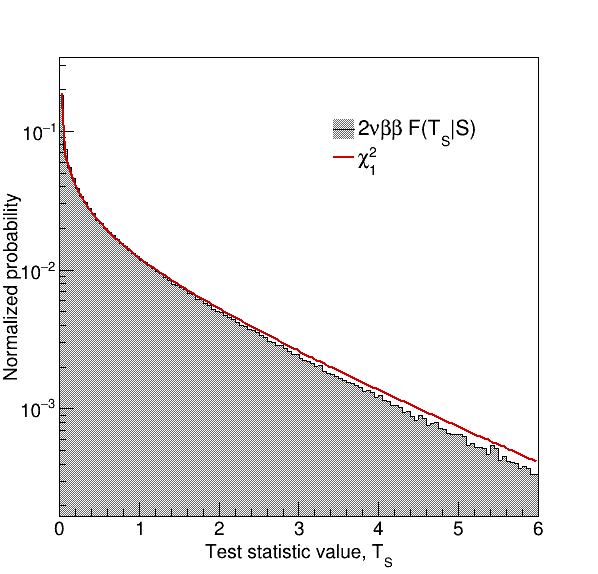
\includegraphics[width=0.4\textwidth]{plots/2nbb-ana/2nbb_teststat.png}%
  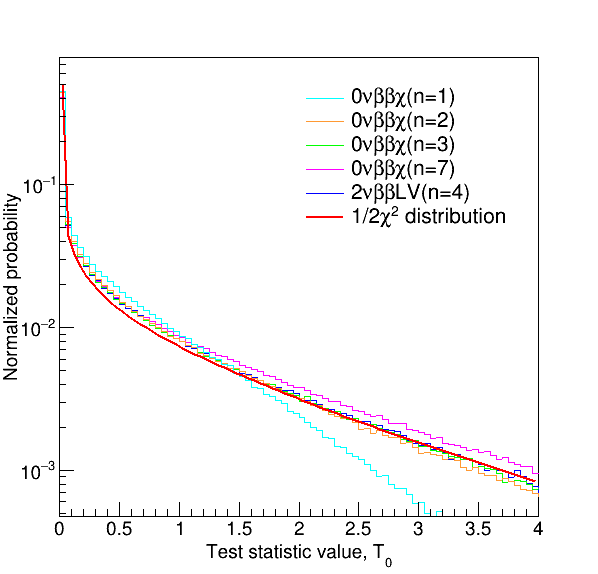
\includegraphics[width=0.4\textwidth]{plots/2nbb-ana/teststatNewphysics.png}
  \caption{%
    \fillme{Betta give me the histos}
  }\label{fig:2nbb-ana:ts-dist}
\end{figure}

\blocktitle{sensitivity \\ studies}
The sensitivity to alternative signal hypotheses can be characterized by the median
significance, assuming data generated according to the zero-signal (null) hypothesis, with
which one rejects the signal hypothesis~\cite{Cowan2011}. To compute the sensitivity the
distributions $f(t_S|S)$ and $f(t_S|0)$ are needed. For a discrete set of hypothesis on
the signal $S$, the two distributions are obtained with Toy Monte Carlo and the median
\pvalue\ assuming the null hypothesis is computed. Figure \cref{fig:?} shows the median
\pvalue\ as a function of $S$, for all the considered processes.  The sensitivity for 90\%
C.L.~limit setting corresponds to the value of $S$ for which the median \pvalue\ is 0.1.
In \cref{tab:2nbb-ana:sensitivity} the sensitivity on the half-lives of the investigated
processes are reported.

\begin{table}
  \centering
  \caption{%
    Statistical-only sensitivity for 90\% C.L.~limit setting on the half-lives of some new
    physics processes contributing to the \nnbb\ event distribution. The results are
    extracted from toy Monte Carlo data sets.
  }\label{tab:2nbb-ana:sensitivity}
  \begin{tabular}{ccc}
    \toprule
    Decay mode             & Spectral index ($n$) & Sensitivity            \\
    \midrule
    \onbbx\                & 1                    & $1.0 \cdot 10^{24}$ yr \\
    \onbbx\                & 2                    & $1.0 \cdot 10^{23}$ yr \\
    $\onbbM\upchi(\upchi)$ & 3                    & $1.0 \cdot 10^{23}$ yr \\
    \onbbxx\               & 7                    & $1.0 \cdot 10^{23}$ yr \\
    \nnbblv\               & 4                    & \fillme{?}             \\
    \bottomrule
  \end{tabular}
\end{table}

\section{Systematic uncertainties}%
\label{sec:2nbb-ana:systematics}

Besides the purely-statistical effects, a set of uncertainties which might contribute
systematically to the final analysis uncertainty (both for the \nnbb\ half-life and
new-physics limits) must be considered. Until now, the test statistics studies have been
considering only the effect of Poisson fluctuations in the bin contents, as the generative
model for the toy data sets was fixed. A way to include systematic model uncertainties
when sampling the test statistic distribution is to sample the generative pdf from a set
of `alternative' models according to a certain probability distribution. This is
conceptually equivalent to fitting the data with `wrong' models that assume the presence
of a systematic distortion of the best model. As instance, alternative transition layer
or LAr veto models induce coherent distortions in all background and signal pdfs, which
must be taken into account when generating the toy data sets.
\newpar
This way of treating systematic uncertainties is formalized as a \emph{hybrid
Bayesian-frequentist} approach~\cite{Tanabashi2018}. In this setting, the distribution
of the test statistic becomes:
\[
  f(t_s) = \int f(t_s | S, \vec{B}, \nu) \pi(\vec{\nu}) d\vec{\nu} \;,
\]
Where $\vec{\nu}$ are the parameters representing the sources of systematic uncertainties
in the model and $\pi(\vec{\nu})$ a `prior' distribution from which $\vec{\nu}$ is sampled
from. The effect introduced by these additional parameters is to smear $f(t_S)$ and
enlarge its tail, weakening the new-physics experimental limits extracted from it. The
software that implements this approach for the \nnbb\ analysis is implemented in the
\texttt{gerda-factor} suite, publicly available on GitHub\footnote{The
\texttt{gerda-factory} software suite: \url{https://github.com/gipert/gerda-factory}.
\fillme{describe}}.

\begin{figure}
  \centering
  \includegraphics{plots/2nbb-ana/bege-pdf-dist.pdf}
  \caption{%
    Distortions
  }\label{fig:2nbb-ana:pdf-dist}
\end{figure}

\begin{description}

  \item[LAr veto model] The Monte Carlo LAr veto model, as shown in detail in
    \cref{sec:bkg:lar:ph2:pdfs}, suffers from many uncertainties, some of them arising
    directly from the poor knowledge of LAr channel efficiencies and material optical
    properties implemented in \mage\ (c.f.r~\cref{sec:apdx:mage-optics}). The systematic
    effect of variations of some of these Monte Carlo parameters (i.e.~the LAr absorption
    length, the germanium reflectivity, the coverage of the fiber shroud and the TPB
    quantum efficiency) has been already studied in selected regions of the LAr
    probability map (the object in which the LAr veto model is encoded) in
    \cref{sec:bkg:lar:ph2:heatmap,fig:bkg:lar:ph2:larmap:dist}. Special calibration data
    can be used to determine the channel efficiencies (\cref{sec:bkg:lar:ph2:pcalib}), but
    could not be exploited to reliably constrain other Monte Carlo parameters. This second
    possibility, which requires a much more complex analysis and a deeper understanding of
    simulated and physics data, is discussed in~\cite{Wiesinger2021}.
    \newpar
    To include the LAr veto model uncertainties in the \nnbb\ distribution analysis, the
    following approach has been formulated. First, the special calibration data is
    compared to Monte Carlo simulations to extract three effective channel efficiencies:
    one for all top PMTs, one for all SiPM modules and one for all bottom PMTs
    (\cref{eq:bkg:lar:ph2:chan-eff}). Considering the cylindrical symmetry of the problem
    (a set of detectors arranged in a cylindrical array), A more detailed knowledge of
    efficiencies for each single channel is not necessary. In this reference probability
    map the other Monte Carlo optical parameters are fixed to the values that better
    reflect our degree of belief, which are documented in \cref{sec:apdx:mage-optics}.
    \newpar
    The second step is to provide alternative LAr veto maps for the determination of the
    test statistic distribution, generated with different assumptions for the optical
    parameters. These alternative maps will still have to reproduce the special
    calibration data (i.e.~they will have to be re-tuned on them), which is, technically
    speaking, the \emph{control sample}, but they will differ from the original map in all
    other LAr regions, in particular those probed by the background source simulations.
    Unfortunately, the map generation process is exceptionally expensive from
    the computational point of view (the required time is on the order of several
    thousands of CPU hours), therefore obtaining several alternative probability maps from
    scratch is not feasible. To overcome with this issue, the possibility to perform
    manual distortions of the reference probability map has been investigated.
    \newpar
    An alternative presentation of the probability map distortions in
    \cref{fig:bkg:lar:ph2:larmap:dist}, in which the detection probability in the first
    calibration source position area is set to unity, is given in
    \cref{fig:2nbb-ana:dist-pcanorm} for the germanium reflectivity, the fiber shroud
    coverage and the LAr absorption length (first three panels from left). In this way the
    constraint of reproducing the special calibration data set is made visually explicit,
    as the corresponding probability (in red) is invariant under transformations of the
    Monte Carlo parameters. TPB quantum efficiency and LAr light yield distortions are not
    considered because they can be well-approximated with a global scaling of the
    probability map (i.e.~their effect is fully absorbed in the LAr channel efficiencies).
    The distortions shown in the rightmost panel are obtained in a different way: instead
    of running the full simulation chain with different Monte Carlo parameters to compute
    the detection probability in the selected spatial points, the probability map is
    directly distorted by means of an analytical transformation. A power-law
    transformation is used:
    \[
      p_k \rightarrow c \cdot p_k^a \;,
    \]
    in which $p_k$ is the probability value in the LAr voxel $k$ (i.e.~the probability
    map) and $a$ is an arbitrary coefficient controlling the magnitude of the distortion
    and $c$ is a constant factor to let the new map reproducing the special
    calibration data. \fillme{the analysis flow is not very logical here, talk with
    Christoph}

    \begin{figure}
      \centering
      \includegraphics{plots/2nbb-ana/larmap-dist-pcanorm.pdf}
      \caption{%
        Study of the impact of Monte Carlo parameters on LAr light detection probabilities in
        various spatial points, normalized to unity at the best value and such to leave the
        probability at the uppermost calibration source position (red point) unchanged. In
        the rightmost panel the effect of a direct, power-law transformation of the
        probability map is shown (no normalization to the red point applied, see text for
        details). The color code and other details are described in
        \cref{fig:bkg:lar:ph2:larmap:dist}.
      }\label{fig:2nbb-ana:dist-pcanorm}
    \end{figure}

  \item[Transition layer model] \fillme{fillme}

  \item[Detector active volume] \fillme{fillme}

  \item[Background model] \fillme{fillme}

  \item[Theoretical \nnbb\ decay model] \fillme{fillme}

  \item[\mage\ and \geant{}] \fillme{fillme}

\end{description}

\section{Results and discussion}

% vim: tw=90
